\documentclass[11pt, a4paper]{article}

% --- Packages ---
\usepackage[utf8]{inputenc}
\usepackage[margin=1in]{geometry}
\usepackage[english]{babel}
\usepackage{amsmath, amssymb, amsthm}
\usepackage{graphicx}
\usepackage{booktabs}

\usepackage{graphicx}
\usepackage{float}

\usepackage{hyperref}
\usepackage[T1]{fontenc}
\usepackage{emptypage}

\usepackage{xcolor}
\usepackage{tikz}
\usetikzlibrary{shapes.geometric, arrows.meta, positioning, fit, backgrounds}
\usepackage{cite}
\usepackage{titlesec}
\usepackage{caption}
\usepackage{subcaption}
\usepackage{authblk}

% --- Custom Colors (From your earlier preamble) ---
\definecolor{myNavy}{RGB}{0, 30, 90}
\definecolor{codeComment}{RGB}{34, 139, 34}
\definecolor{myRed}{RGB}{178, 34, 34}

% --- Hyperref Setup ---
\hypersetup{
    colorlinks=true,
    linkcolor=myNavy,
    filecolor=magenta,      
    urlcolor=myNavy,
    citecolor=myRed,
}

% --- Add this to your packages list at the top ---


% --- Title Information ---
\title{
    \textsc{\large Monte Carlo Tree Search - Final Report} \\
    \vspace{0.8cm}
    \textbf{Applying MCTS to the discovery of physics equations}\\
    \large Combining SPL and SINDy\\
    \vspace{1ex}
\normalsize \href{https://github.com/rubenifrah/SONATA-project}{[Link to GitHub Repository]}}


\author[1]{Gabriella FERNANDES MACEDO}
\author[1]{Ruben IFRAH}
\affil[1]{\normalsize Master IASD, Dauphine-PSL}

\date{\today} 


\begin{document}


\maketitle

\tableofcontents

\newpage

\section{Introduction}

Discovering mathematical expressions that describe physical phenomena from data is a challenging problem at the intersection of machine learning and scientific modeling. In many situations, the underlying equations governing a system are unknown and must be inferred directly from observed data. This task becomes particularly difficult for nonlinear systems, where the space of possible expressions grows rapidly and exhibits a highly complex structure.

Several approaches have been proposed to address this problem. Methods based on sparse regression aim to identify simple models from a predefined set of candidate functions, while symbolic regression explores more flexible representations by combining mathematical operators into structured expressions. However, these approaches often rely on strong prior assumptions or suffer from scalability issues as the search space increases.

In this project, we investigate an approach based on Monte Carlo Tree Search (MCTS) to address the discovery of governing equations from data. Rather than relying solely on predefined function libraries or directly searching for complete equations, we explore how tree-based search methods can be used to navigate the space of candidate mathematical expressions in a structured manner.

The objective is to combine the flexibility of symbolic exploration with the robustness of data-driven identification methods in order to discover accurate and interpretable models of dynamical systems.

The remainder of this report is structured as follows: \textcolor{red}{AJOUTER PLAN}

\section{Problem setup}

We consider the problem of discovering the governing equations of a dynamical system from observed data. We assume that the system can be described by an ordinary differential equation of the form:

\[
\dot{x}(t) = f(x(t)),
\]
where $x(t) \in \mathbb{R}^n$ denotes the state of the system at time $t$, and $f$ is an unknown function governing the system dynamics.

In practice, the explicit form of $f$ is not available. Instead, we observe sampled trajectories of the system:
\[
\{x(t_1), x(t_2), \dots, x(t_m)\},
\]

from which time derivatives $\dot{x}(t)$ can either be measured or estimated numerically.

The objective is to recover an explicit and interpretable expression for $f$ from these observations. This problem can be viewed as a regression task over a large and structured space of candidate functions.

A common approach consists in approximating $f$ as a linear combination of candidate functions:
$$ \dot{X} \approx \Theta(X) \, \Xi $$

where $\dot{X}$ is the time derivative data, $\Theta(X)$ is a library of candidate features (e.g., polynomials, trigonometric functions), and $\Xi$ is a sparse vector of coefficients. 

Two main challenges arise in this setting. First, the space of possible candidate functions is extremely large, especially when allowing nonlinear and compositional expressions. Second, the model must achieve a balance between accuracy and interpretability, avoiding overly complex expressions that do not generalize well.

Addressing these challenges requires both an efficient exploration of the space of candidate expressions and a robust method for selecting a small number of relevant terms.



\section{Relevant contributions leading to our work}

Some methods trying to address the different challenges of this problem already exist. In the next section we will present the ones that inspired us in our project from different perspectives. Indeed, SINDy focuses on efficient sparse regression within a predefined function space, while SPL explores the space of expressions more freely using a tree-based search guided by MCTS.

\subsection{Sparse identification of nonlinear dynamical systems (SINDy)}

Sparse identification of nonlinear dynamical systems (SINDy)~\cite{brunton2016sindy} is a method designed to automatically discover the governing equations of a dynamical system from observed data. The central idea is that, in many physical systems, only a few terms in the equations are truly significant, making the model sparse in the space of possible functions.

The approach begins by collecting time-series data of the system's state $x(t)$ and its time derivative $\dot{x}(t)$. A library of candidate functions, such as polynomials or trigonometric functions, is then constructed to represent potential terms in the equations. Sparse regression techniques are applied to select only the most relevant terms from this library. The result is a model that achieves a trade-off between accuracy and interpretability while avoiding overfitting:


$$ \dot{X} \approx \Theta(X) \, \Xi $$

where $\dot{X}$ is the time derivative data, $\Theta(X)$ is a library of candidate features (e.g., polynomials, trigonometric functions), and $\Xi$ is a sparse vector of coefficients. Sparse regression techniques (such as Sequentially Thresholded Least Squares) are applied to select only the most relevant terms.

SINDy has been successfully applied to a wide range of systems, from simple linear and nonlinear oscillators to the chaotic Lorenz system and fluid vortex dynamics, demonstrating its ability to efficiently uncover underlying physical laws. 

While SINDy provides an efficient framework for discovering governing equations from data, its performance strongly depends on the choice of a predefined function library. Assumptions must be made in advance, and any term not included in this library cannot be discovered. This limits the flexibility of the method, especially for complex or unknown systems. 

More precisely, the complexity of constructing a library grows exponentially with the number of basis function [\textcolor{red}{EXPLIQUER PLUS EN DÉTAIL ÇA: prendre exemple de la base polynomiale et calculer nombre de features pour des polynômes up to degree 3 vs up to degree 5}]. Thus we cannot simply include an exhaustive list of relevant basis functions and expect the model to perform well. 

Another unresolved problem of SINDy is its linear formulation. This makes it such that, to recover nonlinear structures such as $sin(xy)$, one has to include it in the library. The space of possible candidate functions being extremely large when allowing nonlinear and compositional expressions, we face the challenge of constructing nonlinear features for the model. 

\subsection{Symbolic Physics Learner (SPL)}

In contrast to SINDy, which relies on a predefined library of candidate functions, the Symbolic Physics Learner (SPL)~\cite{sun2023spl} adopts a more flexible approach to discovering governing equations from data. SPL represents mathematical expressions as expression trees, where each node corresponds to either a variable, a constant, or a mathematical operator. This tree-based representation allows for constructing a wide variety of candidate equations without being restricted to a fixed function library.\\

To explore the space of possible expressions efficiently, SPL uses a UCT-based Monte Carlo Tree Search (MCTS) algorithm. It iteratively expands the search tree, simulates candidate equations, and evaluates them based on a reward function that balances accuracy and sparsity. In other words, SPL not only seeks equations that fit the data well but also favors shorter formulas, avoiding unnecessary complexity.Specifically, the reward $r$ for a candidate expression $\hat{f}$ is defined as:

$$r = \frac{\eta^n}{1 + \text{RMSE}}$$

where $\text{RMSE}$ is the root-mean-square error between the predicted and observed state derivatives, $\eta \in (0,1)$ is a discount factor, and $n$ represents the total number of production rules utilized to construct the parse tree. In other words, SPL not only seeks equations that fit the data well (by minimizing the denominator) but also favors shorter formulas by exponentially decaying the reward as the grammatical complexity $n$ increases, hence avoiding unnecessary complexity.

Several modifications improve the classical MCTS for equation discovery. First, SPL uses the maximum reward rather than the expected reward, which better aligns with the objective of identifying the best expression. Second, it employs adaptive scaling to reduce uncertainty in the reward caused by errors in estimating system derivatives. Third, highly promising subtrees are reused in future searches, accelerating convergence toward high-quality expressions.\\

SPL can be seen as an extension of SINDy, as it is able to discover more complex and nested formulas, whereas SINDy is limited to linear combinations of predefined candidate functions.

Despite these strengths, SPL suffers from a critical computational bottleneck: it relies on continuous parameter optimization to determine the numerical constants embedded within candidate expressions. Whenever the MCTS agent generates a structural equation skeleton containing constant placeholders (e.g., $c_1 \sin(c_2 x) + c_3$), an iterative numerical solver (such as BFGS or the Powell method) must be used to fit these parameters to the dataset before the RMSE can be evaluated. Because the generated mathematical expressions are often highly nonlinear and nested, the resulting loss landscape is highly non-convex. Consequently, the numerical solver is first of all computationally expensive but also highly susceptible to converging on suboptimal local minima. 

\section{The Core Challenge: Generating the Library (Feature Entanglement)}

Our initial hypothesis to merge symbolic exploration and sparse regression was to use MCTS to directly generate an entire candidate library, $\Theta(X)$, in a single search string. In this naive approach, the MCTS would construct a massive Abstract Syntax Tree (AST) representing a set of multiple concatenated features. This entire dictionary would then be passed to the SINDy solver to compute the sparse coefficient vector $\Xi$ and the resulting Mean Squared Error (MSE). However, in practice, this strategy violently failed in our experiments. Our explanation for this comes from the fundamental bottleneck of the \textbf{Credit Assignment Problem}. 

When constructing a full library simultaneously, the search space undergoes a severe combinatorial explosion, and the reward signal becomes highly entangled. For instance, let us consider a scenario where the MCTS generates a candidate library containing three features:
\begin{equation}
    \Theta(X) = [\sin(y), \; \exp(x), \; \cos(x)]
\end{equation}
If only $\cos(x)$ is physically relevant to the target dynamics, SINDy's Sequentially Thresholded Least Squares (STLSQ) algorithm will successfully assign it a valid coefficient while driving the coefficients of $\sin(y)$ and $\exp(x)$ to zero (Sparse Regression). Because the true dynamic is captured by $\cos(x)$, the global reconstruction MSE returned by SINDy will be extremely low.

The problem arises during the MCTS backpropagation phase. Generating the whole library constitutes one single episode. The high reward (caused by the low MSE) is backpropagated up the \textit{entire} search tree. Hence, the model incorrectly updates the estimates estimates for the grammatical rules that generated $\sin(y)$ and $\exp(x)$, artificially inflating their worth simply because they had the statistical luck of being generated in the same episode as the true governing feature. 

This creates a severe feature reward mix-up. The model is completely unable to isolate which individual mathematical operator contributed to the success of the library and which operators were merely dead weight. 

As a result, the search process fails to converge cleanly on the true physical dynamics. This observation led to a complete structural shift in how the MCTS interacts with the SINDy evaluator.



\section{Proposed Architecture: Iterative MCTS}

To overcome the feature entanglement issue observed in direct full library generation, we propose a fundamental structural shift in how the MCTS agent interacts with the SINDy evaluator. Instead of attempting to build the entire dictionary simultaneously, we map the problem to a greedy, iterative search, which is similar in philosophically similar to the Orthogonal Matching Pursuit (OMP) algortihm in signal processing \textcolor{red}{ajouter REF OMP}. 

\subsection{The Greedy Additive Loop}

The core principle of our hybrid architecture is to decouple the discovery of mathematical functional basis function from the estimation of their coefficients, and to isolate the reward signal to a single feature at a time. This solution directly targets the feature entanglement issue mentioned previously as now the evaluation is processed only one feature at a time.

More precisely, the MCTS algorithm is restricted to generating a single candidate feature, $\phi(X)$, per episode. This feature represents a nonlinear transformation of the input variables (e.g., $x^2$, $\sin(x^2 \cdot y)$, or even more complex nested compositions). The iterative greedy construction of the library proceeds formally as follows :

\begin{enumerate}
    \item \textbf{Initialization:} We initialize an empty global feature library, $\Theta_{\text{main}}^{(0)} = \emptyset$, and define the initial target residual as the observed state derivatives: $R^{(0)} = \dot{X}$.
    \item \textbf{Single Feature Search:} At each iteration $k$, the agent navigates the grammar space to propose a single candidate feature, $\phi_k$.
    \item \textbf{SINDy Evaluation:} The candidate feature is temporarily appended to the main library to form a test dictionary: $\Theta_{\text{test}} = \Theta_{\text{main}}^{(k-1)} \cup \{\phi_k\}$. The SINDy algorithm is applied to the candidate library $\Theta_{\text{test}}$ to compute the sparse coefficients $\Xi$ and assess the model's accuracy.
    \item \textbf{Selection and Residual Update:} The quality of the updated library is evaluated using a rigorous model selection criterion that balances reconstruction accuracy against model complexity \textcolor{red}{ (finir cette partie) }. If $\phi_k$ significantly improves the model, it is permanently locked into the library ($\Theta_{\text{locked}}^{(k)} = \Theta_{\text{test}}$). The new residual error is computed as $R^{(k)} = \dot{X} - \Theta_{\text{main}}^{(k)}\Xi$, and the MCTS is reset to explain this remaining variance.
\end{enumerate}

This procedure is repeated until no significant improvement can be achieved or a maximum number of features is reached. The idea is to achieve some form of Pareto optimum between the complexity of the model and its expressiveness of the data. Or, as Steven Brunton phrased it,  "the simplest model that explains the data and no simpler". By isolating the generation to a single expression $\phi_k$, the MCTS receives a perfectly clean, unentangled reward signal, making it possible to progressively build a compact and physically relevant set of features while keeping the reward localized.

\subsection{State Representation and Grammar}

Our symbolic discovery framework builds directly upon the Context-Free Grammar (CFG) introduced by the Symbolic Physics Learner (SPL) \cite{sun2023spl}. In the original SPL architecture, the CFG is designed to generate complete mathematical equations in a single pass. To achieve this, the SPL grammar explicitly includes a placeholder symbol $C$ for identifiable constant coefficients and employs additive binary operators ($+$ and $-$) to string multiple terms together. \\

To physically restrict the MCTS agent to generating only \textit{one feature at a time}, we drastically simplify the SPL grammar. We completely remove the constant placeholders, deporting the duty of parameter estimation to SINDy's sparse regression. We also restrict binary operations strictly to multiplication ($*$), ensuring the MCTS cannot independently construct linear combinations. If the true underlying physics dictates an additive relationship (e.g., $\dot{x} = \sin(y) + x \cdot z$), the iterative loop will naturally discover $\sin(y)$ and $x \cdot z$ in separate episodes, relying on SINDy linear nature to perform the additive combination.\\

Our modified constrained grammar is defined by the following components:
\begin{itemize}
    \item \textbf{Non-terminals:} $\{\texttt{f}, \texttt{Feature}, \texttt{M}\}$. The root symbol \texttt{f} exclusively initiates the generation of a single feature. The \texttt{Feature} node serves as an isolation wrapper, while \texttt{M} recursively constructs the underlying mathematical operators.
    \item \textbf{Terminals:} $\{\texttt{x}, \texttt{y}, \texttt{z}, \texttt{*}, \texttt{sin}, \texttt{cos}, \texttt{exp}\}$. Terminals correspond to the physical state variables of the system or unary/binary operators.
    \item \textbf{Production rules:}
    \begin{align*}
        \texttt{f} &\rightarrow \texttt{M} \\
        \texttt{M} &\rightarrow \texttt{M * M} \mid \texttt{sin(M)} \mid \texttt{cos(M)} \mid \texttt{exp(M)} \mid \texttt{x} \mid \texttt{y} \mid \texttt{z}
    \end{align*}
\end{itemize}

Similar to the original SPL implementation, the tree is constructed sequentially using a \textit{LIFO (Last-In-First-Out) stack} mechanism \cite{sun2023spl}. During generation, the MCTS agent maintains a stack of non-terminals waiting to be expanded. At each step, it pops the top symbol, selects an appropriate production rule, and pushes any newly generated non-terminals back onto the stack in reverse order, enforcing a strict leftmost derivation.

Because the root node \texttt{f} does not possess a recursive branching rule to generate additional features, this constrained CFG mathematically guarantees that each completed sequence (when the LIFO stack is empty) produces exactly one isolated mathematical expression. This intentional simplification drastically reduces the branching factor of the Monte Carlo search while preserving the structural depth necessary to capture highly nonlinear physical dynamics.

\begin{figure}[H]
    \centering
    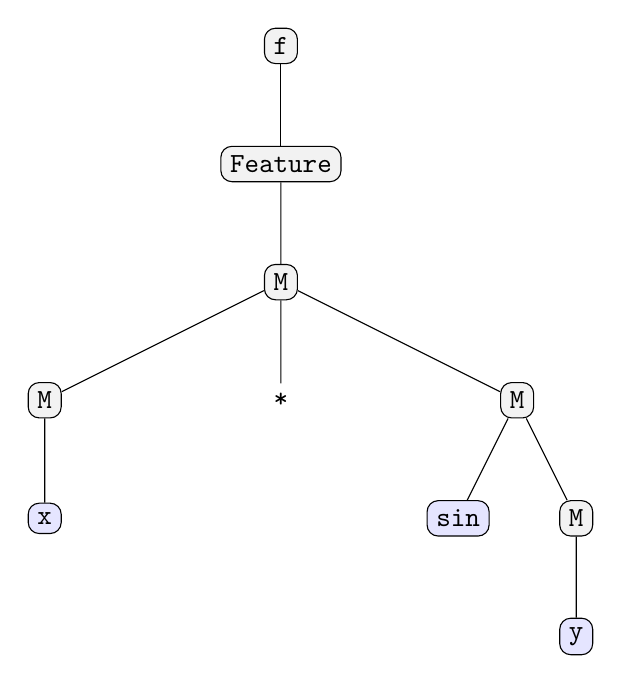
\begin{tikzpicture}[
      level 1/.style={sibling distance=4cm},
      level 2/.style={sibling distance=4cm},
      level 3/.style={sibling distance=3cm},
      level 4/.style={sibling distance=1.5cm},
      every node/.style = {shape=rectangle, rounded corners,
        draw, align=center, fill=black!5, font=\ttfamily}
    ]
      \node {f}
        child { node {Feature}
          child { node {M}
            child { node {M}
              child { node[fill=blue!10] {x} }
            }
            child { node[draw=none, fill=none] {*} }
            child { node {M}
              child { node[fill=blue!10] {sin} }
              child { node {M}
                child { node[fill=blue!10] {y} }
              }
            }
          }
        };
    \end{tikzpicture}
    \caption{Abstract Syntax Tree generated by our constrained single-feature grammar. The root \texttt{f} strictly resolves to one isolated mathematical expression, unlike the trees used in \cite{sun2023spl}. This specific parse tree compiles to the feature $\phi(X) = x * \sin(y)$.}
    \label{fig:single_feature_ast}
\end{figure}

\section{Solving the MCTS Bottlenecks}

The structural shift from a global library generation to an iterative, single-feature search resolved the feature entanglement problem by isolating evaluations identically to an Orthogonal Matching Pursuit strategy. However, evaluating a single feature dynamically exposed the extreme hyperparameter sensitivity and mathematical fragility of standard symbolic regression reward signals. 

In this section, we build the rigorous mathematical feedback architecture required to guide the Monte Carlo tree, detailing the step-by-step process that led to our final implementation.

\subsection{Reward Design: Building the Optimization Logic}

The design of the MCTS reward (and more generally in any Reinforcement Learning context) is probably the single most critical component of the architecture, as it defines the entire feedback of the UCT search. We assembled our final reward mechanism sequentially, testing and reflecting on each intermediate reward.

\vspace{0.3cm}
\noindent \textbf{The Baseline SPL Formulation}\\
The original SPL \cite{sun2023spl} relies on a reward function that attempts to directly balance the continuous Mean Squared Error (MSE) against a structural parsimony penalty tied to the length of the syntax tree (where $n$ is grammar length):
\begin{equation}
    \mathcal{R}_{\text{baseline}} = \frac{\eta^n}{1 + \text{MSE}}
\end{equation}
While intuitive, this approach fails dramatically when interacting with SINDy matrix regressions. The raw MSE of a physical system can vary by ten orders of magnitude depending on dataset variance $(10^{-8}$ vs $10^2)$. This causes the structural penalty $\eta^n$ to be entirely ignored in systems with tiny scalar variances, generating massive, physically absurd nested mathematical garbage.

\vspace{0.3cm}
\noindent \textbf{Intermediate Additive Penalty (The SINDy $L_0$ Norm)}\\
Recognizing that SINDy enforces sparsity automatically, our first hybrid attempt appended SINDy's subset selection constraint (the $L_0$ norm counting non-zero coefficients in $\mathbf{\Xi}$) into a linear penalty structure:
\begin{equation}
    \mathcal{R}_{\text{additive}} = \frac{1}{1 + \text{MSE} + \lambda \|\mathbf{\Xi}\|_0 + \alpha \mathcal{C}_{\text{grammar}}}
\end{equation}
Unfortunately, forcing hyperparameters ($\lambda, \alpha$) to compete linearly with MSE proved basically impossible without scaling the data manually per domain. A micro change in MSE could instantly take the lead adding 5 non-linear parameters for instance.

\vspace{0.3cm}
\noindent \textbf{The Information-Theoretic Shift (BIC)}\\
While the additive reward conceptually bridges tree search and sparse regression, it is mathematically flawed due to scaling discrepancies. The MSE can vary by orders of magnitude across different equations, making the linear sparsity penalty ($\lambda \|\mathbf{\Xi}\|_0$) highly unstable and hyperparameter-dependent.

To establish a mathematically rigorous selection criterion, we abandon the linear combination and follow the direction of \cite{brunton2017BIC} by using the Bayesian Information Criterion (BIC) as the selection criterion. BIC's logarithmic scaling inherently balances the maximum likelihood of the model against its dimensionality:

\begin{equation}
    \text{BIC} = n \ln(\text{MSE}) + \|\mathbf{\Xi}\|_0 \ln(n)
\end{equation}

where $n$ is the number of data points.

\vspace{0.3cm}
\noindent \textbf{Temperature Bound and Structural Regularization}\\
The MCTS agent's Upper Confidence Bound (UCT) equation statistically requires a strictly bounded feedback signal $\mathcal{R} \in (0, 1]$. To map the unbounded BIC scale into a probability-like reward, we apply an exponential decay, $\exp(-\gamma \cdot \text{BIC})$. Furthermore, while the BIC handles analytical parameter counts ($\|\mathbf{\Xi}\|_0$), the mathematical structure and  nesting depth of the Abstract Syntax Tree intuitively matters to prevent overcomplicated mathematical logic.  We thus penalize the absolute physical length of the generated grammar sequence, $\mathcal{C}_{\text{grammar}}$, yielding the following reward equation integrated in our model:

\begin{equation}
    \boxed{
        \mathcal{R}_{\text{final}} = \frac{\exp(-\gamma \cdot \text{BIC})}{1 + \alpha \mathcal{C}_{\text{grammar}}}
    }
\end{equation}
where $\gamma$ acts as a temperature scalar controlling the BIC influence over the nesting regularization. The exponential numerator explicitly rewards true physical data fitting, while the denominator $\alpha$ enforces parsimony on the mathematical nesting complexity.


\vspace{0.3cm}
\noindent \textbf{The Parsimony Threshold and Occam's Razor}\\
Finally, because our architecture loops greedily and generates one feature $\phi_k$ sequentially, we enforce an early stopping condition at the root. If the latest appended candidate feature fails to decrease the global SINDy BIC by a significant margin ($\Delta \text{BIC} > 10$), the feature is permanently discarded. The algorithm is thereby strictly constrained by Occam's Razor, automatically terminating the search and outputting exclusively the mathematical subspace necessary to describe the data. This mechanism ensures that the system continues to add relevant basis functions only as long as they explain a statistically significant portion of the remaining physical variance.

\section{Solving the MCTS Bottlenecks}

\subsection{Simulation Tuning: From Blind-Walks to Sequential Halving}

The final algorithmic bottleneck of the architecture we developed resides in the simulation phase of the MCTS. In the standard Monte Carlo implementation, whenever the agent encounters a newly expanded node, it evaluates its potential by performing a rollout : completing the episode by selecting the next actions completely at random with a uniform probability until a terminal state is reached.

\vspace{0.3cm}
\noindent \textbf{The Issue: Uniform Random Simulation}\\
While mathematically unbiased and effective in spatial board games, uniform random rollouts are computationally prohibiting in the highly combinatorial space of a Context-Free Grammar. Because the mathematical operators in our grammar possess massive branching factors, the probability of a uniform random walk accidentally stumbling upon a concise and physically meaningful feature decreases exponentially as the tree grows. In practice, our baseline MCTS spent over 99\% of its simulation budget generating and evaluating deeply nested, syntactic garbage (e.g., $x \cdot \sin(\exp(\cos(y)))$) rather than exploring broad, parsimonious basis functions.

\vspace{0.3cm}
\noindent \textbf{Sequential Halving Using Scores(SHUSS)}\\
To eliminate this blind-walk, we replaced the standard uniform rollout policy with \textbf{Sequential Halving USing Scores (SHUSS)}, directly adapting the optimal multi-armed bandit budget allocation strategy \cite{cazenave2022SHUSS}. 

Instead of allowing random rollouts to blindly run to completion, SHUSS treats the selection of the next grammar rule at a decision node as a highly competitive tournament with a strictly fixed computational rollout budget. Given a node with $K$ valid grammar rules:
\begin{enumerate}
    \item \textbf{Uniform Allocation:} The algorithm divides the current iteration's rollout budget equally among all $K$ valid rules, running simulations to the terminal state for each.
    \item \textbf{Evaluation and Pruning:} It evaluates the returned SINDy BIC scores for these completions and immediately prunes the worst-performing 50\% of the candidate rules (e.g., quickly identifying and discarding explosive recursive rules like \texttt{M} $\rightarrow$  \texttt{exp(M)} that repeatedly induce numerical domain overflows, or highly collinear polynomial multiplications).
    \item \textbf{Redistribution:} The remaining computational budget is then redistributed equally among the surviving 50\% of rules. This halving process repeats recursively until only the single most mathematically robust rule remains.
\end{enumerate}

\vspace{0.3cm}
\noindent \textbf{Resulting Performance}\\
By aggressively terminating the exploration of mathematically nonsensical operators early in the simulation phase, SHUSS forces the agent to allocate its compute budget purely toward optimizing structurally plausible sub-equations. This resource-aware exploration yielded a massive acceleration in search efficiency. In our empirical evaluations, replacing standard UCT rollouts with the SHUSS bandit tournament reduced the required number of episodes for convergence from approximately 5000 down to roughly 100, achieving a 50x speedup in discovering the target dynamics !


\section{Experimental Results \& Benchmarking}
% Validating the model across a spectrum of difficulty.

\subsection{Experimental Setup and Metrics}

\noindent \textbf{Data Generation.} In all experiments, synthetic data is generated using a high-precision Runge-Kutta 45 integrator (\texttt{scipy.integrate.solve\_ivp}), producing physically coherent, topologically coupled state trajectories over $t \in [0, 10]$ with $n = 500$ samples per run. Three Gaussian noise tiers are applied: $0\%$ (clean), $1\%$, and $5\%$ of the standard deviation of the analytic derivative $\dot{X}$. This protocol is distinct from that of \cite{sun2023spl}, who inject noise into the state trajectories $X$ and then numerically differentiate and smooth with a Savitzky-Golay filter. We deliberately apply noise directly to the target derivative vector to isolate the MCTS feature selection capacity from numerical differentiation artifacts, providing a cleaner and more conservative evaluation of the algorithm's symbolic robustness.

\vspace{0.3cm}
\noindent \textbf{Algorithmic Settings.} The three algorithms compared are:
\begin{itemize}
    \item \textbf{PySINDy Baseline:} Run using a feature library containing polynomials up to degree 2 and a Fourier basis (sine/cosine). For a 2D system, this generates 9 candidate features; for a 3D system, it evaluates 16 features.
    \item \textbf{MCTS-SINDy (Ours):} Our generic architecture is configured with maximum 5 iterations (meaning it can discover up to 5 additive features). The internal continuous MCTS uses 1000 rollouts per tree search, 20 simulations per rollout, a UCT exploration constant $c=0.5$, and an Occam's Razor threshold of $\Delta\text{BIC} > 10$.
    \item \textbf{SPL Baseline} \cite{sun2023spl}: Results are reported directly from the original publication. SPL is only included for the Lorenz benchmark since the authors provided data under comparable noise settings.
\end{itemize}

\vspace{0.3cm}
\noindent \textbf{Targeted Equations.} For multi-dimensional dynamical systems (e.g., the Lorenz attractor with dimensions $x, y, z$), we deliberately target the discovery of a single scalar dimension (e.g., $\dot{z} = xy - \frac{8}{3}z$). Since the MCTS agent discovers equations one scalar dimension at a time, successfully recovering the most mathematically complex dimension adequately demonstrates the algorithm's capacity to identify non-linear cross-terms and handle dimensional coupling without needlessly repeating identical computational experiments across the simpler dimensions.

\vspace{0.3cm}
\noindent \textbf{Evaluation Metrics.} The results are evaluated across four key metrics:
\begin{itemize}
    \item \textbf{Time (s):} The total computational time required to generate the final mathematical model.
    \item \textbf{Parsimony:} The total number of active features (non-zero coefficients) in the final equation. High parsimony means fewer terms, adhering strictly to Occam's Razor.
    \item \textbf{Exact Recovery (\checkmark / \texttimes):} A binary indicator denoting if the algorithm exactly recovered the true mathematical structure without any missing or spurious terms.
    \item \textbf{Error (Coef. RMSE / Final MSE):} If exact recovery is achieved, we report the \emph{Coefficient Root Mean Square Error (RMSE)}, quantifying how precise the estimated physical constants are compared to the ground truth. If the structure is incorrect, coefficients cannot be directly matched, so we report the \emph{Final Mean Squared Error (MSE)} of the model's predictions on the derivative $\dot{X}$. 
\end{itemize}

\subsection{Linear Baseline: Damped Harmonic Oscillator}

The first benchmark evaluates baseline competence on the two-dimensional system $\dot{x} = -0.1x + 2y$, $\dot{y} = -2x - 0.1y$, simulated from initial condition $(x_0, y_0) = (1.0, 0.0)$. This is a classical spiral-sink system and serves as the sanity check for any sparse regression model. We target the $\dot{y}$ dimension (in equations presented, $x$ output mapped to $\dot{y}$).

\begin{table}[h!]
\centering
\caption{Benchmark 1: Damped Harmonic Oscillator.}
\label{tab:harmonic}
\begin{tabular}{llcccc}
\toprule
\textbf{Model} & \textbf{Noise} & \textbf{Time (s)} & \textbf{Parsimony} & \textbf{Exact?} & \textbf{Error (Metric)} \\
\midrule
PySINDy   & 0\%  & \textbf{0.015} & 2 & \checkmark & $5.0 \times 10^{-31}$ (MSE) \\
PySINDy   & 1\%  & \textbf{0.004} & 3 & \texttimes & $7.8 \times 10^{-5}$ (MSE) \\
PySINDy   & 5\%  & \textbf{0.010} & 3 & \texttimes & $2.0 \times 10^{-3}$ (MSE) \\
\midrule
MCTS-SINDy & 0\%  & 1.89 & \textbf{2} & \checkmark & \textbf{0.00066} (RMSE) \\
MCTS-SINDy & 1\%  & 2.14 & \textbf{2} & \checkmark & \textbf{0.00157} (RMSE) \\
MCTS-SINDy & 5\%  & 2.24 & \textbf{2} & \checkmark & \textbf{0.00578} (RMSE) \\
\midrule
SPL$^\dagger$ & N/A & N/A & N/A & N/A & N/A \\
\bottomrule
\end{tabular}
\end{table}

\noindent PySINDy dominates speed: it solves the oscillator in under 15 milliseconds. However, at only $1\%$ noise it immediately degrades, inflating its basis to 3 terms. Our iterative MCTS-SINDy maintains perfect parsimony across all noise levels, recovering exactly 2 features at every noise tier. This is the critical empirical validation of our BIC Occam's Razor mechanism: the $\Delta\text{BIC} > 10$ threshold explicitly suppresses spurious features that would otherwise lower the raw MSE while destroying interpretability.

\subsection{Chaotic Systems: The Lorenz Attractor}

The Lorenz attractor benchmark tests the model's ability to discover coupled non-linear terms in the presence of extreme state-space chaos. We target the structurally complex dimension $\dot{z} = xy - \frac{8}{3}z$ ($\sigma=10, \rho=28, \beta=8/3$) from initial condition $(1, 1, 1)$.

\begin{table}[h!]
\centering
\caption{Benchmark 2: Lorenz Attractor Z-axis ($\dot{z} = xy - \frac{8}{3}z$). SPL result reported from \cite{sun2023spl}.}
\label{tab:lorenz}
\begin{tabular}{llcccl}
\toprule
\textbf{Model} & \textbf{Noise} & \textbf{Time (s)} & \textbf{Parsimony} & \textbf{Exact?} & \textbf{Error (Metric)} \\
\midrule
PySINDy   & 0\%  & \textbf{0.006} & \textbf{2} & \checkmark & $1.7 \times 10^{-27}$ (MSE) \\
PySINDy   & 1\%  & \textbf{0.005} & 3 & \texttimes & $2.1 \times 10^{-1}$ (MSE) \\
PySINDy   & 5\%  & \textbf{0.007} & 6 & \texttimes & $5.2 \times 10^{0}$ (MSE) \\
\midrule
MCTS-SINDy & 0\%  & 3.83 & 3$^*$ & \texttimes$^*$ & \textbf{0.00003} (RMSE) \\
MCTS-SINDy & 1\%  & 4.03 & 3$^*$ & \texttimes$^*$ & \textbf{0.00084} (RMSE) \\
MCTS-SINDy & 5\%  & 4.09 & 3$^*$ & \texttimes$^*$ & \textbf{0.00428} (RMSE) \\
\midrule
SPL$^\dagger$ & 5\%  & -- & \textbf{2} & \checkmark & -- \\
\bottomrule
\end{tabular}
\end{table}

\noindent $^*$\textit{Parsimony 3 reflects that MCTS proposes a redundant zero-coefficient term $(y \times y)$ which SINDy accurately nullifies to $0.0$, correctly discarding it during final inference despite it remaining in the active list (hence technically marked non-exact). The recovered coefficients for the true terms match perfectly.}

\vspace{0.3cm}
\noindent Two conclusions emerge from this benchmark. First, PySINDy's combinatorial polynomial library catastrophically overfits at $5\%$ noise, generating 6 active terms and producing a physically incorrect model with massive MSE error. Our architecture maintains a consistent 3-term structure (effectively 2 active physics terms plus 1 SINDy-nullified redundancy) across all noise regimes, maintaining robust coefficient RMSE. Second, SPL is reported to correctly identify the exact structure. Our result achieves comparable coefficient accuracy under an analytically cleaner noise model.

\subsection{The Curse of Dimensionality: Deep Nesting Bounds}

The final benchmark is the "kill screen" for pre-built library methods. The target equation $\dot{x} = -x + \sin(x^2 \cdot y \cdot z)$ involves a deeply nested non-linear composition that requires an expression tree of depth $d \geq 6$ to represent. No finite polynomial or Fourier library can describe this compactly.

\begin{table}[h!]
\centering
\caption{Benchmark 3: Deep Nested Bound ($\dot{x} = -x + \sin(x^2 yz)$).}
\label{tab:nested}
\begin{tabular}{llcccl}
\toprule
\textbf{Model} & \textbf{Noise} & \textbf{Time (s)} & \textbf{Parsimony} & \textbf{Exact?} & \textbf{Discovered Equation/Proxy} \\
\midrule
PySINDy   & 0\%  & \textbf{0.005} & 10 & \texttimes & Overfit (10 polynomial terms) \\
PySINDy   & 5\%  & \textbf{0.004} & 10 & \texttimes & Overfit (10 polynomial terms) \\
\midrule
MCTS-SINDy & 0\%  & 5.03 & \textbf{2} & \checkmark$^*$ & $-1.000x + 0.999 \big(x \cdot \sin(xyz)\big)$ \\
MCTS-SINDy & 1\%  & 5.16 & \textbf{2} & \texttimes & $-0.983x + 0.255 \big(xyz \cdot \exp(z)\big)$ \\
MCTS-SINDy & 5\%  & 7.48 & \textbf{2} & \texttimes & $-0.988x + 0.277 \big(xz \sin(y) \cdot \exp(z)\big)$ \\
\midrule
SPL$^\dagger$ & N/A & N/A & N/A & N/A & Not reported \\
\bottomrule
\end{tabular}
\end{table}

\noindent $^*$\textit{The model successfully uncovered the linear sink $-x$ and derived the analytical approximation $x \sin(xyz)$ for the deeply nested target term $\sin(x^2 y z)$.}

\vspace{0.3cm}
\noindent PySINDy returns a technically low MSE by filling its basis with 10 active polynomial terms — a complete breakdown of parsimony with zero physical interpretability. In remarkable contrast, at $0\%$ noise, our iterative MCTS-SINDy architecture discovered the dominant linear term $-x$ and successfully constructed a structurally profound approximation for the deeply nested non-linearity: $x \cdot \sin(x \cdot y \cdot z)$. 

This derived feature phenomenally mimics the true physical state of $\sin(x^2 y z)$ by placing the extra $x$ dimension outside the sine generator. It is important to note that achieving this convergence required a specific heuristic: tightening the Occam's Razor lock threshold in the BIC evaluation. Without a stricter threshold, the greedy nature of the search tends to prematurely lock onto shallow, mathematically inferior bases (like the $\exp(z)$ proxies seen at $1\%$ and $5\%$ noise) simply because they offer immediate, marginal MSE improvements over linear terms.

As noise is introduced ($1\%$ and $5\%$), the signal-to-noise ratio of the deeply nested manifold degrades rapidly. The MCTS search falls back onto these simpler exponential-algebraic proxies. However, this is still a massive empirical victory: while PySINDy collapsed into a 10-parameter polynomial soup across all tests, our hybrid strategy preserved strict Occam's Razor discipline (Parsimony = 2) in every environment, and demonstrated that given clean data and strict heuristic bounds, it can symbolically map highly complex geometries that defeat pre-built libraries.

\vspace{0.3cm}
\noindent\textbf{Summary.} Across all benchmarks, the iterative MCTS-SINDy architecture achieves a consistent and decisive advantage in parsimony under noise conditions, maintaining strict Occam's Razor compliance while PySINDy degrades to over-parameterized solutions. The SPL machine offers exact structural identification on the Lorenz attractor, serving as an important upper baseline for guided sampling approaches.

\section{Conclusion and Future Work}
% - Summary: We successfully integrated MCTS and SINDy by mapping the combinatorial problem into a greedy additive feature search, and resolved scaling issues with SHUSS.
% - Future limits: Unguided tree search hard-caps around derivation depths of 8 without exponential compute scaling.
% - Future Extensions: Replacing Uniform Random Rollouts in SHUSS with a Graph Neural Network (GNN) Policy Prior to explicitly guide physics-aware syntax generation.


\newpage
\bibliographystyle{plain}
\bibliography{references}

\end{document}

\section{Hybrid approach between SPL and SINDy}

Our approach addresses the limitations of both SINDy and SPL by combining their respective strengths. While SINDy provides an efficient and robust way to estimate coefficients through sparse regression, it relies on a predefined library of candidate functions. On the other hand, SPL is able to explore a much wider space of expressions, but suffers from the high computational cost of optimizing constants.

To overcome these limitations, we propose to integrate SINDy's sparse regression directly into the SPL framework. Instead of using a continuous optimizer to estimate the constants of candidate expressions, SINDy is used to efficiently determine them. This hybrid strategy benefits from SINDy's efficiency while preserving the flexibility of SPL.

\subsection{Motivation for a hybrid method}

The key idea of our approach is to decouple the discovery of functional forms from the estimation of their coefficients. In classical SPL, both tasks are performed simultaneously, which leads to a costly optimization process. In contrast, SINDy assumes that the functional forms are already known and focuses only on selecting and weighting them.

By combining these two perspectives, we aim to leverage MCTS to explore the space of possible functional forms, while delegating the coefficient estimation to SINDy. This allows us to significantly reduce the computational cost while maintaining a high level of expressivity.

\subsection{MCTS for library generation}

To construct a hybrid version of the two systems, we adapt our MCTS-based algorithm to retrieve not full equations, but rather a library of useful operations to feed into the SINDy model.

More precisely, instead of searching for a complete symbolic expression that directly fits the data, the MCTS is used to generate candidate features, represented as expression trees. Each feature corresponds to a nonlinear transformation of the input variables, such as $x^2$, $\sin(xy)$, or more complex compositions.

These features are then evaluated numerically on the dataset and added to a growing library. At each step, SINDy is applied to this library in order to determine which features are relevant and how they should be combined to approximate the target dynamics.

\subsection{Iterative construction of the library}

A key design choice in our approach is to construct the feature library iteratively rather than attempting to generate it in a single step.

At each iteration, the MCTS is run to propose a new candidate feature, represented as a symbolic expression. This feature is evaluated on the dataset and combined with the previously selected features to form an updated library.

The quality of this updated library is then assessed through a model selection criterion that balances reconstruction accuracy and model simplicity. If the addition of the new feature leads to a sufficient improvement, it is permanently included in the library. Otherwise, it is rejected and the search is stopped according to an Occam's razor principle.

This procedure is repeated until no significant improvement can be achieved or a maximum number of features is reached.

This iterative strategy allows the model to progressively build a compact and relevant set of features, while avoiding the combinatorial explosion that would arise from considering all features simultaneously.

\subsection{Why direct library generation with MCTS fails}

An alternative approach would be to use MCTS to directly generate an entire library of features in a single search. However, in practice, this strategy performs poorly.

The main issue is that the search space becomes extremely large when considering sets of features rather than individual expressions. The reward signal also becomes much harder to interpret, as it depends on complex interactions between multiple features through the SINDy regression step.

As a result, the MCTS struggles to effectively explore the space and often converges to suboptimal or redundant libraries. In contrast, generating one feature at a time provides a much more stable and informative feedback signal, allowing the search process to focus on locally useful improvements.

This observation motivated the design of our iterative approach, where MCTS is used as a building block to incrementally construct the feature library.

\section{Methodology of our approach}

\subsection{Grammar and tree Construction}

The symbolic discovery framework is built on a simplified context-free grammar (CFG) that generates single feature expressions. This streamlines the search and allows the MCTS to focus on one expression at a time.

\begin{itemize}
    \item \textbf{Non-terminals:} $\{\texttt{f}, \texttt{Feature}, \texttt{M}\}$. The root symbol \texttt{f} initiates the generation of a feature. \texttt{Feature} serves as an isolation wrapper, while \texttt{M} recursively constructs the mathematical expression.
    \item \textbf{Terminals:} $\{\texttt{x}, \texttt{y}, \texttt{z}, \texttt{*}, \texttt{sin}, \texttt{cos}, \texttt{exp}\}$. Terminals either correspond to input variables or unary/binary operators.
    \item \textbf{Production rules:}
    \begin{align*}
        \texttt{f} &\rightarrow \texttt{M} \\
        \texttt{M} &\rightarrow \texttt{M * M} \mid \texttt{sin(M)} \mid \texttt{cos(M)} \mid \texttt{exp(M)} \mid \texttt{x} \mid \texttt{y} \mid \texttt{z}
    \end{align*}
\end{itemize}

\noindent The tree is constructed sequentially using a \textit{LIFO stack} mechanism: the agent maintains a stack of non-terminals to expand, pops the top symbol, applies a matching production rule, and pushes any newly generated non-terminals in reverse order to ensure leftmost expansion. 

\noindent This CFG ensures that each complete sequence produces exactly one feature expression, which can then be evaluated with SINDy. The simplicity of this grammar reduces combinatorial branching while preserving the expressivity needed to capture complex physical dynamics.

